\documentclass[11pt]{report}
\usepackage{pgf}
\usepackage{tikz}
\usetikzlibrary{arrows,automata}
\usepackage[utf8]{inputenc}
 \usepackage{listings}
 \usepackage{color}
 \usepackage{fancyhdr}
 \usepackage{graphicx}
 \usepackage{amsmath}
\pagestyle{fancy}
 \usepackage{comment} 

 \lhead{Geoffrey PERRIN \\ Océane DUBOIS}
 \rhead{MI01 - TP02 : VHDL séquentiel}
 \rfoot{}



\definecolor{dkgreen}{rgb}{0,0.6,0}
\definecolor{gray}{rgb}{0.5,0.5,0.5}
\definecolor{mauve}{rgb}{0.58,0,0.82}

\lstset{frame=tb,
  language=vhdl,
  aboveskip=3mm,
  belowskip=3mm,
  showstringspaces=false,
  columns=flexible,
  basicstyle={\small\ttfamily},
  numbers=none,
  numberstyle=\tiny\color{gray},
  keywordstyle=\color{blue},
  commentstyle=\color{dkgreen},
  stringstyle=\color{mauve},
  breaklines=true,
  breakatwhitespace=true,
  tabsize=3
}

 
%Gummi|065|=)
\title{\textbf{TP02 - VHDL séquentiel}
\author{Geoffrey PERRIN \\ Océane DUBOIS\\}
\date{}}

\begin{document}

\maketitle

\newpage


\section{Compteur de 2 bits}

Dans cet exercice on cherche à implémenter le  modèle VHDL d'un compteur synchrone à 2 bits, 
On utilisera : \begin{itemize}
	 \item  une entrée  pour le reset : PB\_1. Cette entrée est un bouton poussoir qui remet le compteur à '0' si on le met à '1'.
	\item un signal d'entrée (un bouton) PB\_0 , un autre bouton poussoir,qui incrémente le compteur lorsqu'on le met à 1.
	 \item le signal LED\_10 comme signal de sortie, qui est un groupe de 2 led qui permet d'afficher le resultat du compteur.
	 
	\end{itemize}

\medskip

Chaque fois que l'on appuie sur le bouton, le compteur est incrémenté de 1. Le résultat est affiché grâce aux LED. Si la valeur du compteur dépasse 3, le compteur est remis à 0 car la carte affiche le résultat du compteur modulo 4(car on ne peut afficher que 4 chiffres sur les 2 LED). Sinon le bouton reset (PB\_1), permet de remettre le compteur à 0.

\medskip

On pensera à se synchroniser sur le front montant de l'horloge.

\subsection{ Ecriture du programme en VHDL}

Voici le programme de l'exercice 1. On a supprimé les premières instructions dans un soucis de clareté du programme.

Voici d'abord le code du reset synchrone. On a ici un reset synchrone car le signal du reset n'est pas dans la liste de sensibilité du process et qu'il ne prend effet que si le signal PB\_0 change d'état et passe à 1.

\begin{lstlisting}
entity compteur is
PORT(PB_0,PB_1:IN BIT;
		LED_10: OUT INTEGER RANGE 0 to 3);
end compteur;

architecture Behavioral of compteur is

begin
PROCESS(PB_0)
VARIABLE resultat:INTEGER range 0 to 3 := 0;
BEGIN
	IF(PB_0'EVENT and PB_0='1') THEN
		IF PB_1 = '0' THEN 
			resultat := resultat + 1;
		ELSE
			resultat := 0;
		END IF;
	END IF;

LED_10 <= resultat;

END PROCESS;

end Behavioral;

\end{lstlisting}

Et voici maintenant le code du reset asynchrone. On a simplement passé le signal du reset dans la liste de sensibilité du process et on peut activer le reset indépendemment du signal PB\_0, puisque l'activation du reset ne se trouve plus à l'intérieur de la condition "IF(PB\_0'EVENT and PB\_0='1') THEN". Il peut donc se déclancher indépendamment de l'activation du compteur. 


\begin{lstlisting}
entity compteur is
PORT(PB_0,PB_1:IN BIT;
		LED_10: OUT INTEGER RANGE 0 to 3);
end compteur;

architecture Behavioral of compteur is

begin
PROCESS(PB_0, PB_1)
VARIABLE resultat:INTEGER range 0 to 3;
BEGIN
IF (PB_1 = '1') THEN
	resultat := 0;
ELSE IF(PB_0'EVENT and PB_0='1') THEN

			resultat := resultat + 1;
end if;
END IF;

LED_10 <= resultat;

END PROCESS;

END Behavioral;

\end{lstlisting}

Une fois que les deux programmes sont écrits on procède à la synthèse des programmes. 

 \subsection{ Synthèse du code VHDL }
 
La synthèse nous permet d'obtenir 2 schémas : RTL et Technology. Le schéma RTL est celui qui se rapproche le plus du code VHDL. Il est composé de boites, représentants des multiplicateurs, additionneurs, compteurs ... Ces boîtes peuveunt être reliées entre elles par des portes logiques AND, OR ...  On y voit pas de composants physiques. 
 
 Voici le schéma RTL avec le code du reset synchrone :

 \begin{figure}[h]
\begin{center}
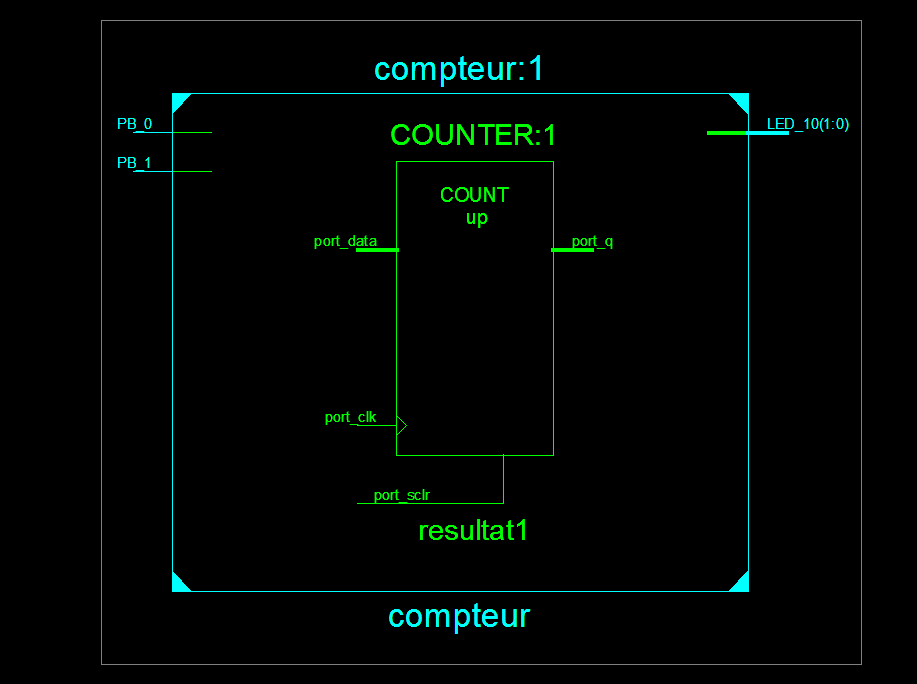
\includegraphics[width=8cm]{TP02-3.PNG}
\caption{Schéma RTL du compteur avec reset synchrone}
\end{center}
\end{figure}


On remarque bien les deux entrée PB\_0 et PB\_1, le compteur au milieu du composant et la LED\_10 qui correspond à la sortie. Le syntéhtiseur à donc bien reconnu le code comme étant un compteur.

Voici maintenant la vue technologique du code avec le reset synchrone : 

\begin{figure}[h!]
\begin{center}
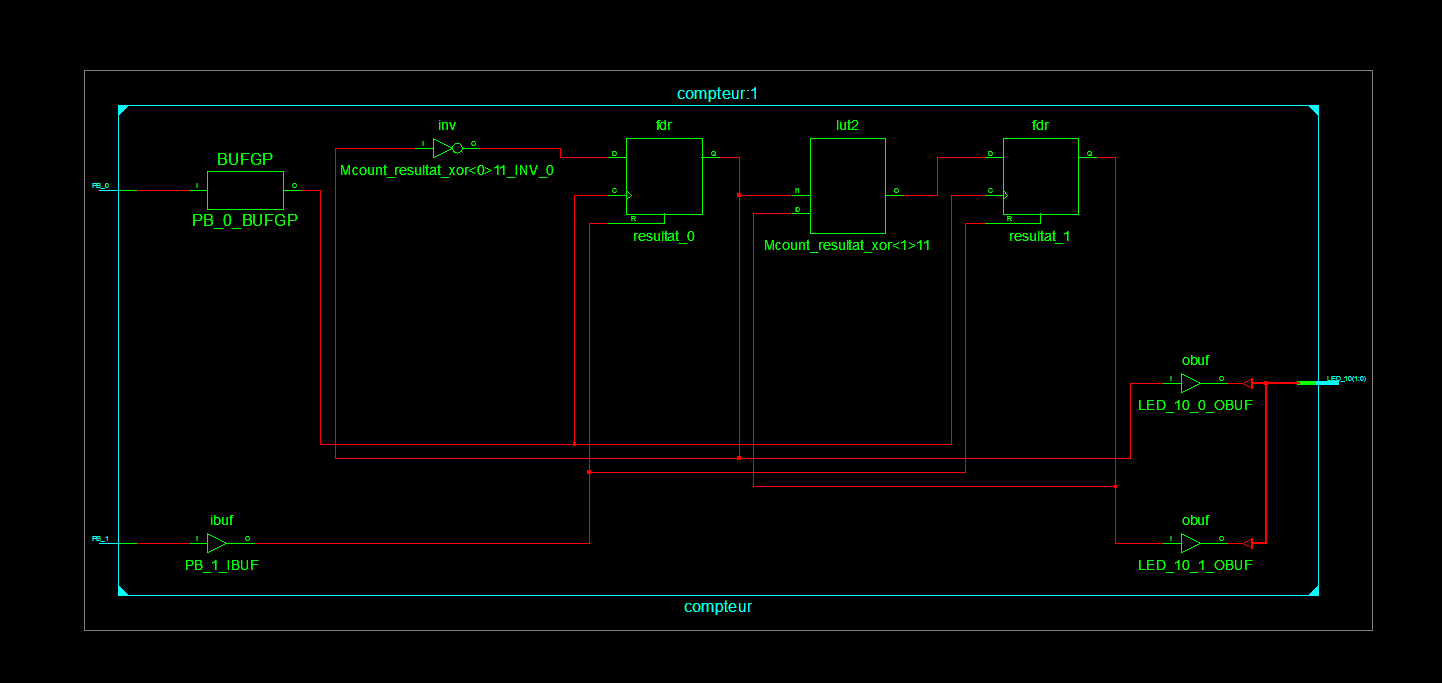
\includegraphics[width=15cm]{TP02-4.PNG}
\caption{Schéma technologique du compteur avec reset synchrone}
\end{center}
\end{figure}

Au niveau de la sortie on a bien les 2 LED qui sont présentes. Le résultat de la LED 0 est calculé par le bloc fdr resultat\_0, le résultat de la led 1 est calculé par le bloc fdr resultat\_1. 
Le reset (l'entrée PB\_1) est reliée à ces 2 même blocs pour les remettre à 0 si besoin. 
C'est le bloc lut2 qui lorsque le bloc fdr resultat\_0 ne peut plus calculer sur 1 bit le résultat, passe le résultat au bloc fdr resultat\_1. 

Tous les composants apparaissant sont des composants qui existent réellement sur le FPGA. 

\newpage
 
\subsection{ Simulation du circuit}

Ensuite nous effectuons la simulation du circuit grâce au logiciel. 
En faisant varier les 2 signaux d'entrée voici le résultat que nous obtenons.

\begin{figure}[h]
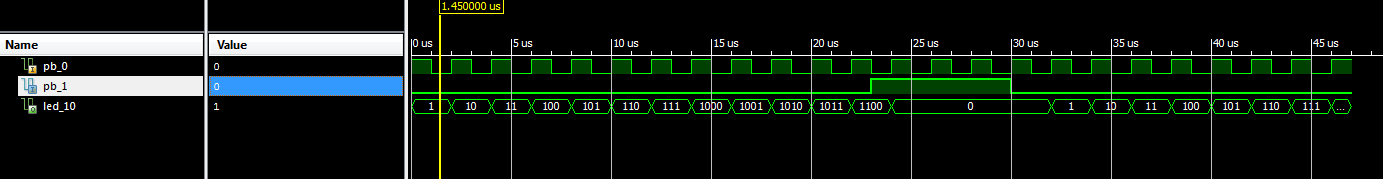
\includegraphics[width=15cm]{TP02-1.PNG}
\caption{Simulation du compteur avec reset synchrone}
\end{figure}

Lors de la simulation avec l'horloge synchrone on remarque que lorsque le reset est activé, on doit attendre que le signal d'entrée PB\_0 soit passé à '1' pour que le compteur repasse à 0, tant que le signal d'entre PB\_0 n'est pas passé à 1, le reset ne prend pas effet.

Ce n'est pas le cas avec un reset asynchrone, dont voici la simulation :

\begin{figure}[h]
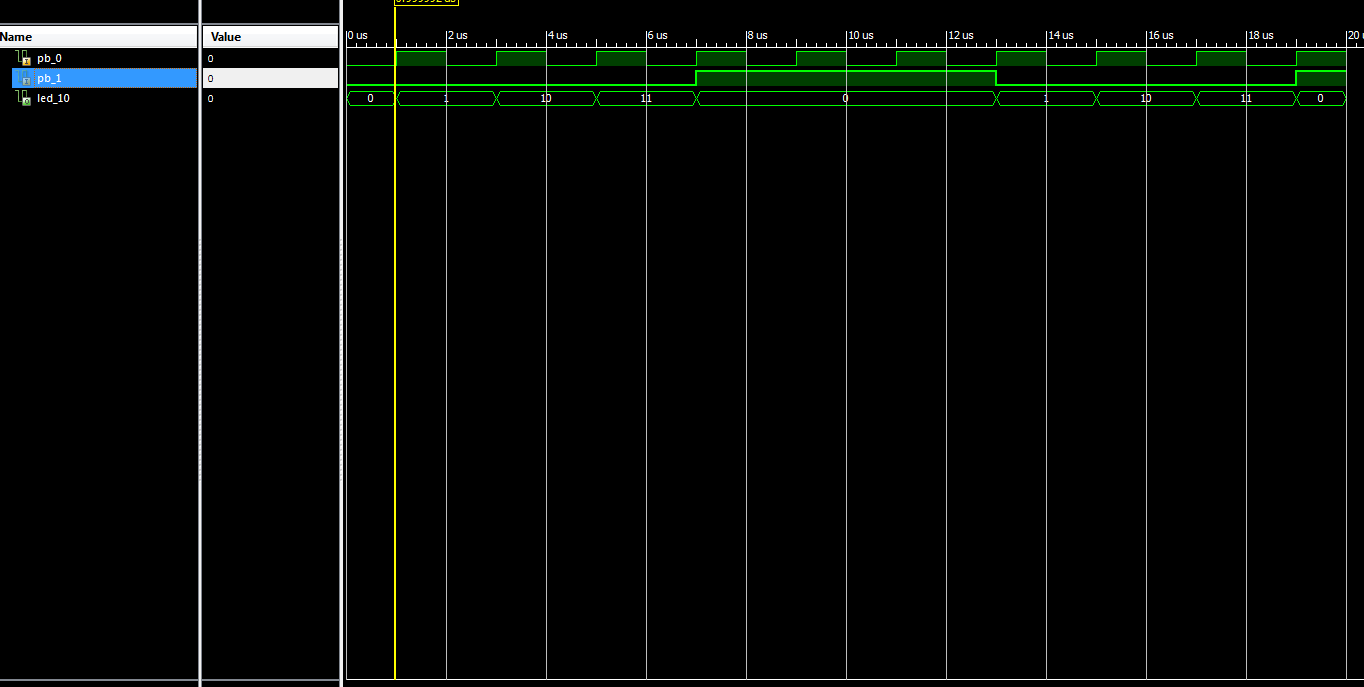
\includegraphics[width=15cm]{TP02-5.PNG}
\caption{Simulation du compteur avec reset asynchrone}
\end{figure}

Ici on peut voir que le reset prend effet dès sont activation, on n'a pas besoin que PB\_0 soit activé. 

  
   \subsection{programmation du FPGA et vérification du fonctionnement}
   
   Lorsqu'on programme le FPGA et qu'on télécharge le code sur la carte, on observe bien les 2 comportements attendus avec les reset synchrone et asynchrone. 
   De plus les 2 leds ne peuvent afficher que les résultats allant de 0 à 3. Une fois que le compteur dépasse la valeur 3, le résultat est affiché modulo 4. 
   

   
 

\section{Détecteur de code}

Dans cet exercice on réalisera un détécteur pour le code 11010. Si le code est détecté, une alarme est activée. On utilisera les signaux :
\begin{itemize}
	\item BP\_0 pour l'horloge
	\item SW\_0 pour la ligne de transmission permettant de rentrer 0 ou 1
	\item LED\_0, la LED pour symboliser l'alarme
	\item LED\_7654 pour afficher l'état de la machine à état

\end{itemize}

Dans cette première modélisation on supposera qu'une fausse entrée implique de tout recommencer. 

On décide de modéliser le code par une machine à 5 états avec chaque état correspondant à une bonne entrée du code.


\begin{comment}
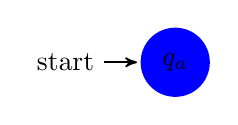
\begin{tikzpicture}[->,>=stealth',shorten >=1pt,auto,node distance=2.8cm,
                    semithick]

	\tikzstyle{every state} = [fill=blue, draw=none, text = black]
	
	\node [initial, state] (1)			{$q_a$};
	
	

\end{tikzpicture}

\end{comment}

\subsection{Ecriture du code VHDL}

\begin{lstlisting}

entity decodeur is
	PORT(PB_0, SW_0 : IN BIT;
		LED_0 : OUT BIT;
		LED_7654 : OUT INTEGER RANGE 0 to 15);
end decodeur;

architecture Behavioral of decodeur is
begin
process(PB_0)
variable state : INTEGER RANGE 0 to 15;
begin
 if(PB_0'Event and PB_0 = '1') then
  case state is
   when 0 => if (SW_0 = '1') then 
      			state := 1; 
      			LED_0 <= '0'; 
			else LED_0 <= '0';
       		end if;
   when 1 => if (SW_0 = '1') then 
      			state := 2; 
       		else
       			LED_0 <= '0'; 
      			state :=0; 
      		end if;
   when 2 => if (SW_0 = '0') then 
      			state := 3; 
			else 
       			LED_0 <= '0';
        		 state :=0; 
      		 end if;
   when 3 => if (SW_0 = '1') then 
    			state := 4; 
       		else
         		LED_0 <= '0'; 
         		state :=0; 
       		end if;
   when 4 => if (SW_0 = '0') then 
     			 state := 0; 
				LED_0 <= '1';
			else 
     			state :=0;
     		end if;
  when others => state := 0;
  end case;
 LED_7654 <= state;
 end if;
end process;
end Behavioral;



\end{lstlisting}

Dans ce code, nous nous sommes basés sur un diagramme à 5 états (de 0 à 4). A chaque entrée qui correpond au code à executer, on incrémente la variable state, si il y a une fausse entrée, on repasse la variable state à 0 et on doit recommencer le code depuis le début. Lorsqu'on arrive à l'état 4 et que le dernier chiffre du code est correctement rentré, on passe la led à 1 pour quelle s'allume. On passe également l'état à 5 pour que lors du cycle suivant, on passe dans la condition "WHEN OTHERS" qui remet l'état à 0. De plus à chaque état nous avons ajouté l'instruction qui permet d'éteindre la LED si le chiffre rentré n'est pas le bon. Nous sommes ainsi sûrs que la LED ne s'allume que si le code correct est rentré et qu'elle s'éteint dans toutes les autres situations. 

Nous égalisons la variable d'état avec le groupe de LED 7654, cela nous permet de savoir à quel état de la machine à état nous sommes, dans l'entrée du code. 


\subsection{ Synthèse du code VHDL }


Nous avons ensuite réalisé la simultaion RTL et Technology du code, voilà ce que nous avons obtenu.



\begin{figure}[!h]
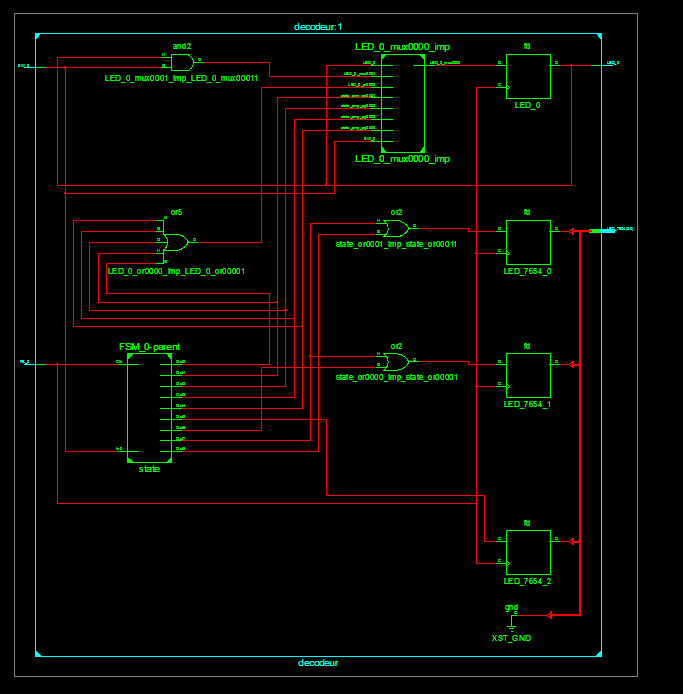
\includegraphics[width=10cm]{TP02-9.PNG}
\caption{Schéma Technology du détecteur, une fausse entrée implique de recommencer du début}
\end{figure}


Nous pouvons donc voir les 3 LED utilisées en sortie pour afficher l'état en plus de la LED\_0 pour afficher l'alarme. 

Pour signal d'horloge, la valeur entrée passe dans un opérateur ET avec le résultat de l'alarme. Puis le résultat des 2 est dirigé vers le bloc LED\_mux\_0.


A la sortie du bloc state il y a aussi une ligne pour chaque état, de l'état 0 à l'état 4. Ces 5 lignes sont dirigée vers le bloc LED\_mux\_0
Ces 5 lignes passent aussi dans un OR, donc la sortie est aussi dirigée vers le bloc LED\_mux\_0.

Le bloc LED\_mux\_0 qui gère donc l'alarme prend donc en entrée les valeurs de states, le signal d'horloge ET le résultat de l'alarme, et la valeur de l'horloge.

Le bloc qui gère la variable state à en sortie une ligne qui se dirige vers chaque LED qui representent la variable state pour les remettre mettre à jour au fur et à mesure.

Il y a aussi une ligne qui rejoins toutes les LED du circuit. Ainsi lorsque l'état 4 est atteint on peut allumer la LED d'alarme. 

Et comme déjà dit, une ligne de sortie par valeur de la variable d'état.

Les bits d'états sont au nombre de 6, sur le schéma RTL ils sont représentés par la notation ouX avec X un entier variant entre 0 et 5.

  
\begin{figure}[!h]
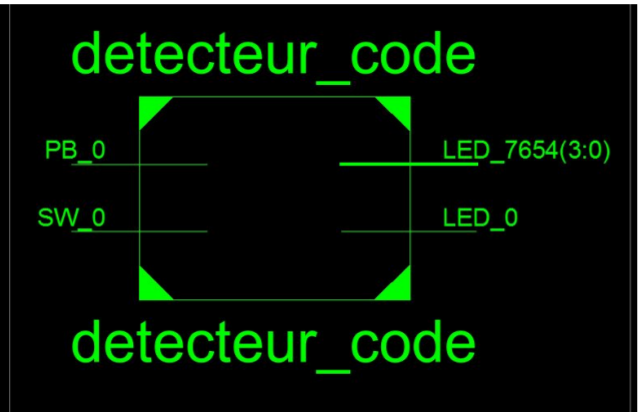
\includegraphics[width=7cm]{TP02-12.png}
\caption{Schéma RTL du détecteur}
\end{figure}


\begin{figure}[!h]
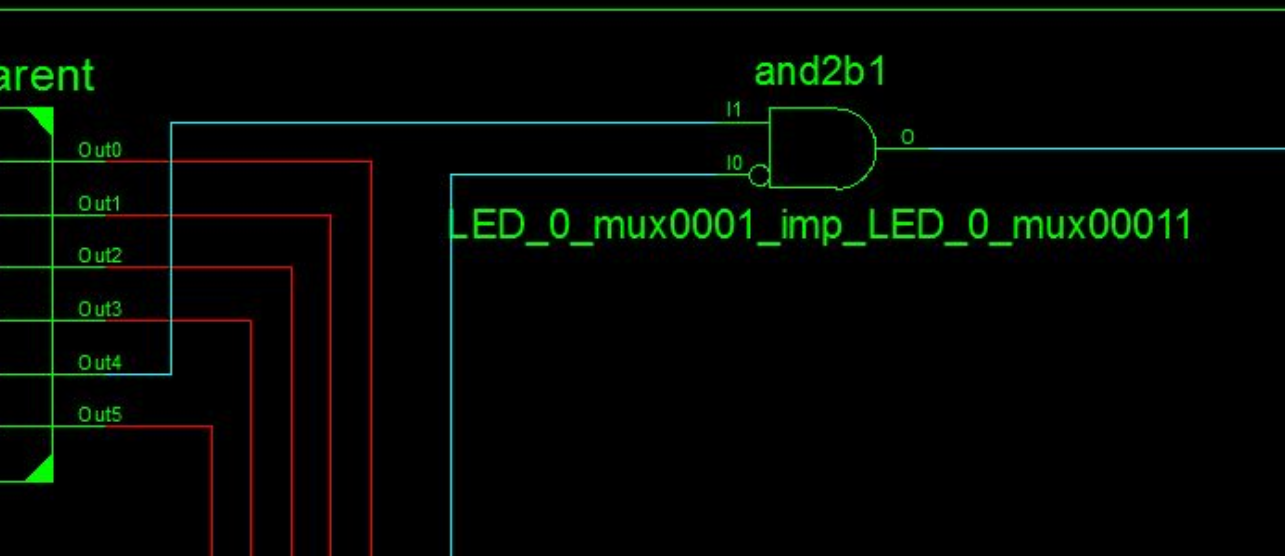
\includegraphics[width=9cm]{TP02-11.png}
\caption{Schéma RTL du détecteur, bit d'états}
\end{figure}
  
  
  On définit : 
  \begin{itemize}
	\item S0 : Out0
	\item S1 : Out1
		\item S2 : Out2
		\item S3 : Out3
		\item S4 : Out4
		\item S5 : Out5

\end{itemize}

D'après le schéma RTL on peut définir les équations de sorties. 
  
 Au niveau des équations de sorties on a donc : \medbreak
 LED\_0 = S4 AND SW\_0 \medbreak 
 LED\_7654(0) = (LED\_7654(3) AND S5) OR (SW\_0 AND S3)\medbreak
 
 LED\_7654(1) = (LED\_7654(2) AND S5) OR (S2 AND SW\_0) \medbreak
 
 LED\_7654(2) = (LED\_7654(1) AND S5) OR (SW\_0 AND S1) \medbreak
 
 LED\_7654(3) = (LED\_7654(0) AND S5) OR (SW\_0 AND S0) \medbreak
 
 
 Ces équations semblent être cohérentes avec le VHDL. Par exemple pour LED\_0, on effectue le ET booléen sur S4 et SW\_0 ce qui correspond au VHDL.  Cependant, les équations de sortie du groupe de LED 7654 font aussi intervenir les valeurs des autres LED, qu'on ne connait pas forcément. Ces équations vérifient également qu'on ne soit pas dans un état incohérent.
  
 
  \subsection{ Simulation du circuit}
 
Lors de la simulation, voici ce que nous avons obtenu, on remarque donc bien que dès qu'une fausse entrée est entrée, la variable d'état retombe à 0. 

\begin{figure}[!h]
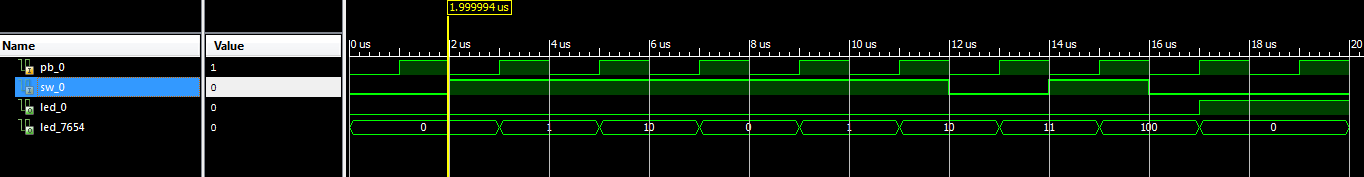
\includegraphics[width=15cm]{TP02-7.PNG}
\caption{Simulation du décodeur, un fausse entrée fait recommencer du début}
\end{figure}
  
  
   \subsection{ programmation du FPGA}

Nous avons donc programmé le FPGA et tout à fonctionné correctement. La machine à état progresse d'état en état à chaque entrée correcte. Ou retombe à 0 si une fausse entrée est mise. 

\section{Détecteur de code avec une fausse entrée négligée}

Dans cet exercice on réalisera un détécteur pour le code 11010. Si le code est détecté, une alarme est activée. On utilisera les signaux :
\begin{itemize}
	\item BP\_0 pour l'horloge
	\item SW\_0 pour la ligne de transmission
	\item LED\_0 pour symboliser l'alarme
	\item LED\_7654 pour afficher l'état

\end{itemize}

Dans cette première modélisation on supposera qu'une fausse entrée est négligée. 

\subsection{Ecriture du code VHDL}

Voici le code VHDL pour le décodeur du code 11010 lorsqu'on néglige une fausse entrée.

\begin{lstlisting}
entity decodeur is
	PORT(PB_0, SW_0 : IN BIT;
		LED_0 : OUT BIT;
		LED_7654 : OUT INTEGER RANGE 0 to 15);
end decodeur;

architecture Behavioral of decodeur is
begin
	process(PB_0)
	variable state : INTEGER RANGE 0 to 5;
	begin
	if(PB_0'Event and PB_0 = '1') then
		case state is
			when 0 => if (SW_0 = '1') then 
						state := 1; 
						LED_0 <= '0'; 
					end if;	
			when 1 => if (SW_0 = '1') then 
						state := 2; 
					else 
						LED_0 <= '0'; 
						state :=1; 
					end if;
			when 2 => if (SW_0 = '0') then 
						state := 3; 
					else 
						LED_0 <= '0';
						state :=2; 
					end if;
			when 3 => if (SW_0 = '1') then 
						state := 4; 
					else
						LED_0 <= '0'; 
  						state :=3; 
					end if;
			when 4 => if (SW_0 = '0') then 
						state := 5; 
					else LED_0 <= '0'; 
						state :=4;
					end if;
			when others => state := 0;
		end case;
	
		LED_7654 <= state;
	end if;
	end process;
end Behavioral;

\end{lstlisting}

On a donc, comme précédement mis l'instruction $LED\_0  \leftarrow'0'$, pour être sûrs que la LED est éteinte. De plus dans le "ELSE", nous avons écrit l'instruction permettant de maintenir l'état à sa valeur actuelle. 



\subsection{ Synthèse du code VHDL }


\begin{figure}[!h]
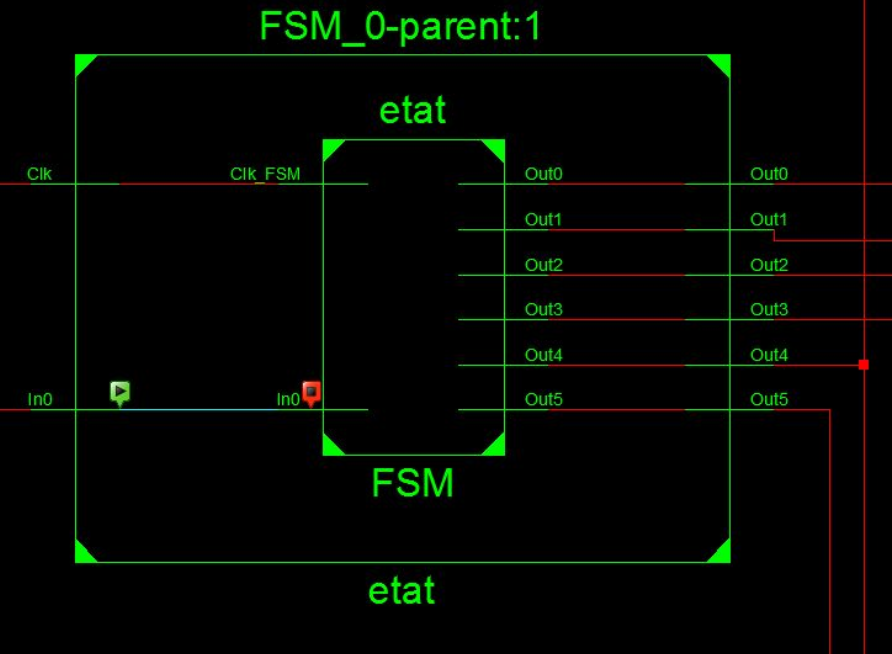
\includegraphics[width=10cm]{TP02-13.png}
\caption{Schéma RTL du décodeur en négligeant une fausse entrée}
\end{figure}

On a toujours le même nombre de bit d'états, soit 6. Cependant les équations de sorties sont plus compliquées et font intervenir beaucoup plus de signaux. 

Si on suppose $LED\_0_t$ l'état de LED\_0 à l'instant t. 
On a : \medbreak
 $LED\_0_t =  (((LED\_0_{t-1} ET (SW\_0)) OR (NOT SW\_0) ET (OUT4)) \\ OU (LED\_0_{t-1} ET (NOT SW\_0)) ET (OUT\_3)) \\ OU (LED\_0_{t-1} ET (SW\_0) ET (OUT\_2)) \\ OU ((( LES\_0_{t-1} ET (SW\_0)) OR (NOT SW\_0)) ET (OUT1)) \\ OU (((LED\_0_{t-1} ET (SW\_0)) OR (NOT SW\_0)) ET (OUT0))$

 Le schéma Technology est également très différent et beaucoup plus complexe. Voici par exemple le circuit qui gènere la sortie LED\_7654(0)
 
 \begin{figure}[!h]
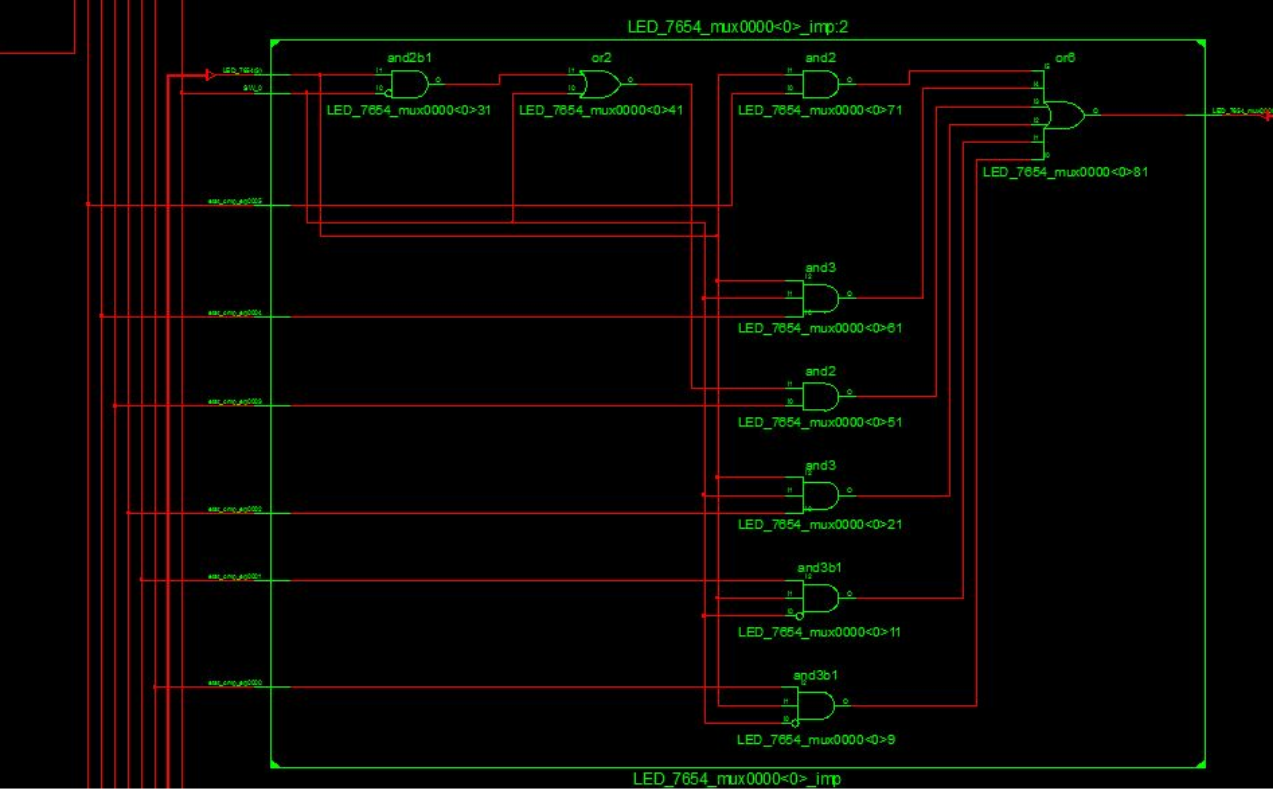
\includegraphics[width=10cm]{TP02-15.png}
\caption{Schéma Technology qui génère la sortie de la LED\_7654(0)}
\end{figure}
 

\end{document}





























